% Uncomment this to make slides with overlays:
%\documentclass[slides]{beamer}

% Uncomment these (but comment the above \documentclass line) to make handouts:
\documentclass[handout]{beamer}

% Uncomment these to have more than one slide per page
%\usepackage{pgfpages}
%\pgfpagesuselayout{2 on 1}[border shrink=5mm]
%\pgfpageslogicalpageoptions{1}{border code=\pgfusepath{stroke}}
%\pgfpageslogicalpageoptions{2}{border code=\pgfusepath{stroke}}

\usepackage[]{graphicx, color, hyperref}

\mode<presentation>
{
	%\usetheme[secheader]{Boadilla}
	%\usecolortheme[rgb={.835, .102,.169}]{structure}  
	\usetheme[width= 0cm]{Goettingen}
	%\setbeamercovered{transparent}
}
\setbeamertemplate{navigation symbols}{}
\setbeamertemplate{footline}[frame number]

\definecolor{blue2}{rgb}{0.278,0.278,0.729} 
\newcommand{\blue}[1]{\textcolor{blue2}{#1}}
\newcommand{\white}[1]{\textcolor{white}{#1}}
\newcommand{\red}[1]{\textcolor{red}{#1}}
\newcommand{\xbar}{\overline{x}}
\newcommand{\ybar}{\overline{y}}
\newcommand{\phat}{\widehat{p}}
\newcommand{\prob}{\mbox{Pr}}
\newcommand{\E}{\mathbb{E}}
\newcommand{\Var}{\mbox{Var}}
\newcommand{\cp}{\oplus}
\newcommand{\cm}{\circleddash}


\title{Lecture 29: Bayesian Statistics}
\author{Chapter 2.2.7}
\date{}


\begin{document}
%------------------------------------------------------------------------------
\begin{frame}
\titlepage
\end{frame}
%------------------------------------------------------------------------------



%------------------------------------------------------------------------------
\begin{frame}
\frametitle{Recall Conditional Probability}

%
% Comment this
%
The \blue{conditional probability} of an event $A$ given the event $B$, is defined by
\[
P(A|B) = \frac{P(A \mbox{ and } B)}{P(B)}
\]  

\end{frame}
%------------------------------------------------------------------------------



%------------------------------------------------------------------------------
\begin{frame}
\frametitle{New Notation}

%
% Comment this
%
Two possible outcomes for hypothesis test:
\begin{itemize}
\item ``reject $H_0$ in favor of $H_A$'' $=$ $\cp$'ve result
\item ``do not reject $H_0$'' $=$ $\cm$'ve result.
\end{itemize}
\pause
\vspace{0.5cm}

with performance measures:
\begin{itemize}
\item $\alpha=0.05=\prob(\mbox{Reject } H_0 \mbox{ when $H_0$ true}) = \prob(\cp|H_0)$
\item Power $=1-\beta=0.8=\prob(\mbox{Reject } H_0 \mbox{ when $H_A$ true}) = \prob(\cp|H_A)$
\end{itemize} 

\end{frame}
%------------------------------------------------------------------------------



%------------------------------------------------------------------------------
\begin{frame}
\frametitle{Previously}

%
% Comment this
%
Say $H_A$ is true 10\% of the time.

\vspace{0.25cm}

So 
\begin{itemize}
\item $\prob(H_A)=0.1$
\item $\prob(H_0) = 1- \prob(H_A) = 1-0.1=0.9$
\end{itemize}
\pause
\vspace{0.25cm}

We conduct 1000 hypotheses of $H_0$ vs $H_A$, so
\begin{itemize}
\item $H_A$ is true 100 times
\item $H_0$ is true 900 times
\end{itemize}



\end{frame}
%------------------------------------------------------------------------------



%------------------------------------------------------------------------------
\begin{frame}
\frametitle{Previously}

So recall from previously we have the following $2 \times 2$ table of possible outcomes:   

\begin{center}
  \begin{tabular}{cc|cc}
     \multicolumn{2}{c}{}  & \multicolumn{2}{c}{\textbf{Test conclusion}} \\ 
     &  & $\cm$ & $\cp$ \\ 
\hline
    \textbf{Truth} & $H_0$ true & $(1-0.05) \times 900 =  855$ & $0.05 \times 900 = 45$ \\
     & $H_A$ true & $(1-0.8)\times 100=20$ & $0.8\times 100= 80$\\ 
    \hline
  \end{tabular}
\end{center}

%
% Comment this
%
\begin{itemize}
\pause\item Of the $\cp$'s, what prop'n was right?\\
i.e. What is $\prob(H_A|\cp)$? \ $\frac{80}{80+45} = 64\%$?  
\pause\item Of the $\cm$'s, what prop'n was right?\\
i.e. What is $\prob(H_0|\cm)$? \ $\frac{855}{855+20} = 97.7\%$
\end{itemize}

\end{frame}
%------------------------------------------------------------------------------



%------------------------------------------------------------------------------
\begin{frame}
\frametitle{Different Set-Up}
Now say for the same machine $H_A$ is true 40\% of the time. i.e. $P(H_A)=0.4$
\pause
\begin{center}
  \begin{tabular}{cc|cc}
     \multicolumn{2}{c}{}  & \multicolumn{2}{c}{\textbf{Test conclusion}} \\ 
     &  & $\cm$ & $\cp$ \\ 
\hline
    \textbf{Truth} & $H_0$ true & $(1-0.05) \times 600 = 570$ & $0.05 \times 600 = 30$ \\
     & $H_A$ true & $(1-0.8)\times 400=80$ & $0.8\times 400= 320$\\ 
    \hline
  \end{tabular}
\end{center}

%
% Comment this
%
\begin{itemize}
\pause\item Of the $\cp$'s, what prop'n was right?\\
$\prob(H_A|\cp) = \frac{320}{320+30} = 91.4\%$?  
\pause\item Of the $\cm$'s, what prop'n was right?\\
$\prob(H_0|\cm) = \frac{570}{570+80} = 87.7\%$
\end{itemize}

\end{frame}
%------------------------------------------------------------------------------


%------------------------------------------------------------------------------
\begin{frame}[fragile]
\frametitle{How Reliable Are Your Test Results?}

%
% Comment this
%
For the \blue{exact same} hypothesis testing machine we get
\begin{center}
  \begin{tabular}{c|cc}
    \hline
    & $\prob(H_A|\cp)$ & $\prob(H_0|\cm)$ \\ 
    \hline
    $P(H_A)=10\%$ & 64\% & 97.7\% \\ 
    $P(H_A)=40\%$ & 91.4\% & 87.7\% \\ 
    \hline
  \end{tabular}
\end{center}

\end{frame}
%------------------------------------------------------------------------------



%------------------------------------------------------------------------------
\begin{frame}[fragile]
\frametitle{How Reliable Are Your Test Results?}

The probability that a positive result is right depends on how likely $H_A$ is.  Same goes for negative results.  

\vspace{0.5cm}

\pause\blue{Question 2 from Quiz 9}: (Nature article) Say a scientist obtains a p-value of 0.01.  An incorrect interpretation of this is that it is the probability of a ``false alarm'' (type I error)...  If one wants to make a statement about this being a false alarm, what additional piece of information is required?\\

\vspace{0.5cm}

\pause\blue{Answer 2}: The plausibility of the hypothesis being tested for.  


\end{frame}
%------------------------------------------------------------------------------



%------------------------------------------------------------------------------
\begin{frame}[fragile]
\frametitle{Bayes Theorem}

%
% Comment this
%
This brings us to Bayes Theorem: 
\pause\begin{itemize}
\item Let $A_1, \ldots, A_k$ be $k$ events that are a \blue{partition} of the sample space $S$.
\item Let $B$ be an event of interest
\end{itemize}
\pause
\vspace{0.5cm}

The Bayes Theorem states: 
\[
\prob(A_i|B) = \frac{\prob(B|A_i)\times\prob(A_i)}{\sum_{j=1}^{k}\prob(B|A_j)\times\prob(A_j)} 
\]

\end{frame}
%------------------------------------------------------------------------------


%------------------------------------------------------------------------------
\begin{frame}[fragile]
\frametitle{Illustration}

\begin{itemize}
\item The sample sample $S$ is the overall grey box
\item $A_1, \ldots, A_5$ are the five blocks that partition $S$.  
\item $B$ is the oval
\end{itemize}

\begin{center}
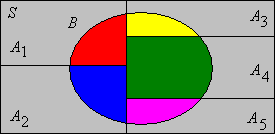
\includegraphics[width=0.8\textwidth]{figure/lotp.png} 
\end{center}

\end{frame}
%------------------------------------------------------------------------------


%------------------------------------------------------------------------------
\begin{frame}[fragile]
\frametitle{Tailored to our Situation}

%
% Comment this
%
\begin{itemize}
\item The sample sample $S$ is all possible hypotheses
\item $H_0$ and $H_A$ partition $S$.  i.e. $k=2$
\item Let $B$ be a $\cp$ result
\end{itemize}
\pause
Then by Bayes Theorem, the probability that a $\cp$ result is right is
\begin{eqnarray*}
\prob(H_A|\cp) &=& \frac{\prob(\cp|H_A)\prob(H_A)}{\prob(\cp|H_A)\prob(H_A) + \prob(\cp|H_0)\prob(H_0)} \\
\pause &=& \frac{(1-\beta)\times\prob(H_A)}{(1-\beta)\times\prob(H_A) + \alpha\times\prob(H_0)}\end{eqnarray*}

Notions of \blue{both} type I error rate and power (AKA type II error rate) are included!

\end{frame}
%------------------------------------------------------------------------------


%------------------------------------------------------------------------------
\begin{frame}[fragile]
\frametitle{Tailored to our Situation}

%
% Comment this
%
Back to initial example where $\alpha=0.05$, $1-\beta=0.8$, $\prob(H_A)=0.10$
\pause
\begin{eqnarray*}
\prob(H_A|\cp) &=& \frac{0.8 \times 0.1}{0.8 \times 0.1 + 0.05\times 0.9} = 0.64
\end{eqnarray*}

\pause Similarly
\begin{eqnarray*}
\prob(H_0|\cm) &=& \frac{\prob(\cm|H_0)\prob(H_0)}{\prob(\cm|H_A)\prob(H_A) + \prob(\cm|H_0)\prob(H_0)} \\
&=& \frac{(1-\alpha)\times\prob(H_0)}{
\beta\times\prob(H_A) + (1-\alpha)\times\prob(H_0)}\\
&=& \frac{0.95 \times 0.9}{0.2\times 0.1 + 0.95 \times 0.9} = 0.977\\
%----------
\end{eqnarray*}

\end{frame}
%------------------------------------------------------------------------------



%------------------------------------------------------------------------------
\begin{frame}[fragile]
\frametitle{The Debate}

Previously, you applied Bayes Theorem from scratch/intuition.
\pause
\vspace{0.5cm}

Why isn't everybody taking into account $P(H_A)$ when testing $H_0$ vs $H_A$?
\pause
\vspace{0.5cm}

In this example, we assumed we \blue{knew} the true $P(H_A)$.  In real life however, we don't.


\end{frame}
%------------------------------------------------------------------------------



%%------------------------------------------------------------------------------
%\begin{frame}[fragile]
%\frametitle{Philosophical Schools of Thought (My Understanding)}
%
%Philosophy for dummies:
%\begin{itemize}
%\pause\item \blue{(Logical) Positivism}:  %philosophy of science based on the view that information derived from logical and mathematical treatments and reports of sensory experience is the \blue{exclusive source of all authoritative knowledge}, and that there is valid knowledge (truth) only in scientific knowledge. \blue{The only truth is what we can observe}.
%The only truth/knowledge is what we can observe.
%\pause\item \blue{Subjectivism}:  ``our own mental activity is the only unquestionable fact of our experience''
%\end{itemize}
%
%\end{frame}
%%------------------------------------------------------------------------------



%%------------------------------------------------------------------------------
%\begin{frame}[fragile]
%\frametitle{Probability (Backbone of Statistics)}
%What does probability even mean?
%
%\begin{itemize}
%\pause\item \blue{Positivist View - Frequentist Probability}:  an event's probability is the limit of its relative frequency in a large \blue{observable} number of trials.
%\pause\item \blue{Subjectivist View - Bayesian Probability}:  a subjective measure of the \blue{degree of belief} of the individual assessing the uncertainty of a particular situation.
%\end{itemize}
%
%\pause
%Think
%\begin{itemize}
%\item flipping a coin
%\item rolling a die
%\end{itemize}
%  vs 
%\begin{itemize}
%\item ``The forecast called for a 60\% chance of rain.''
%\item ``I'd say there is a 20\% chance Jamie will be late.''
%\end{itemize}
%
%\end{frame}
%%------------------------------------------------------------------------------



%------------------------------------------------------------------------------
\begin{frame}[fragile]
\frametitle{Statistics In General}
Statistics is inferring about some unknown parameter $\theta$.

\begin{itemize}
\pause\item \blue{Frequentist Statistics}:  the true $\theta$ is a single value.
\pause\item \blue{Bayesian Statistics}:  the true $\theta$ is a \blue{distribution} of values that reflects our \blue{belief} in the plausibility of different values.
\end{itemize}
 
\pause Ex: Coin Flips

\end{frame}
%------------------------------------------------------------------------------


%------------------------------------------------------------------------------
\begin{frame}
\frametitle{The Bayesian Procedure}
To express our belief about $\theta$ from as a Bayesian, we have:
\begin{enumerate}
\pause\item A prior distribution $\prob(\theta)$.  It reflects our \blue{prior} belief about $\theta$.
\pause\item The likelihood function $\prob(X | \theta)$.  This is the mechanism that generates the \blue{data}.
\pause\item A posterior distribution $\prob(\theta | X)$.  We \blue{update} our belief about $\theta$ after observing data $X$.
\[
\prob(\theta | X) = \frac{\prob(X | \theta) \cdot \prob(\theta)}{\prob(X)}
\]
\end{enumerate}
\end{frame}
%------------------------------------------------------------------------------


%------------------------------------------------------------------------------
\begin{frame}
\frametitle{The Issue:  The Bayesian Procedure}

Where do you come up with $\prob(\theta)$?  It's completely \blue{subjective}!  You decide!

\end{frame}
%------------------------------------------------------------------------------




%------------------------------------------------------------------------------
\begin{frame}
\frametitle{Prior Distribution}
This distribution can reflect someone's \blue{prior belief} of $p$.  

\begin{center}
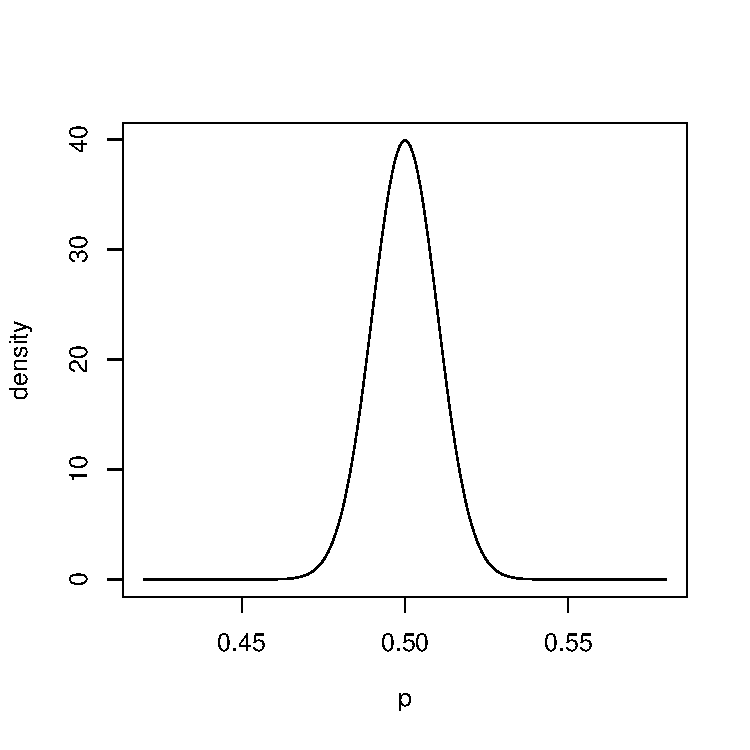
\includegraphics[height=0.7\textheight]{figure/prior.pdf} 
\end{center}

\end{frame}
%------------------------------------------------------------------------------



%------------------------------------------------------------------------------
\begin{frame}
\frametitle{Prior Distribution}
Say someone is more skeptical that $p=0.5$, we can lower it.  

\begin{center}
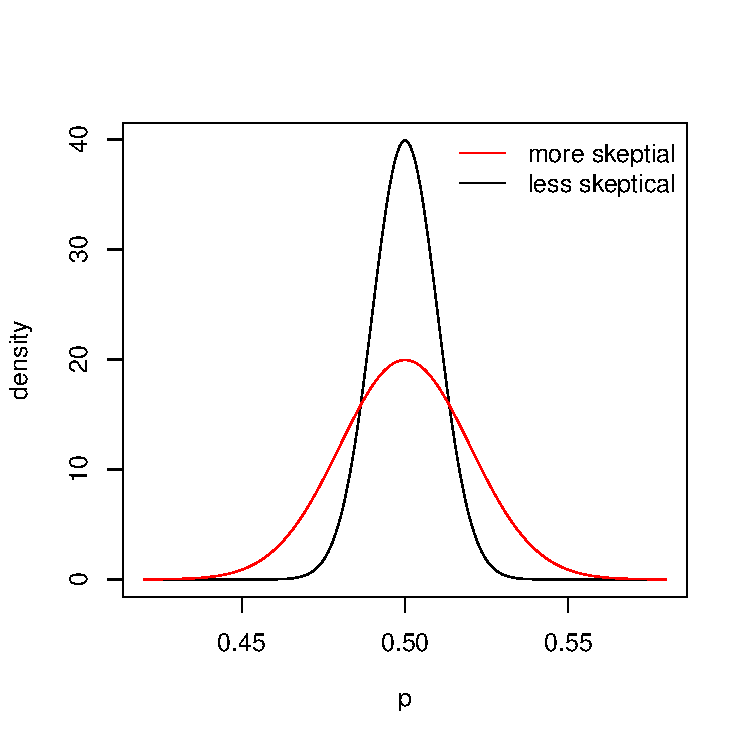
\includegraphics[height=0.7\textheight]{figure/prior2.pdf} 
\end{center}

\end{frame}
%------------------------------------------------------------------------------



%------------------------------------------------------------------------------
\begin{frame}
\frametitle{The Bayesian Procedure}
Say we have the following prior belief centered at $p=0.5$
\begin{center}
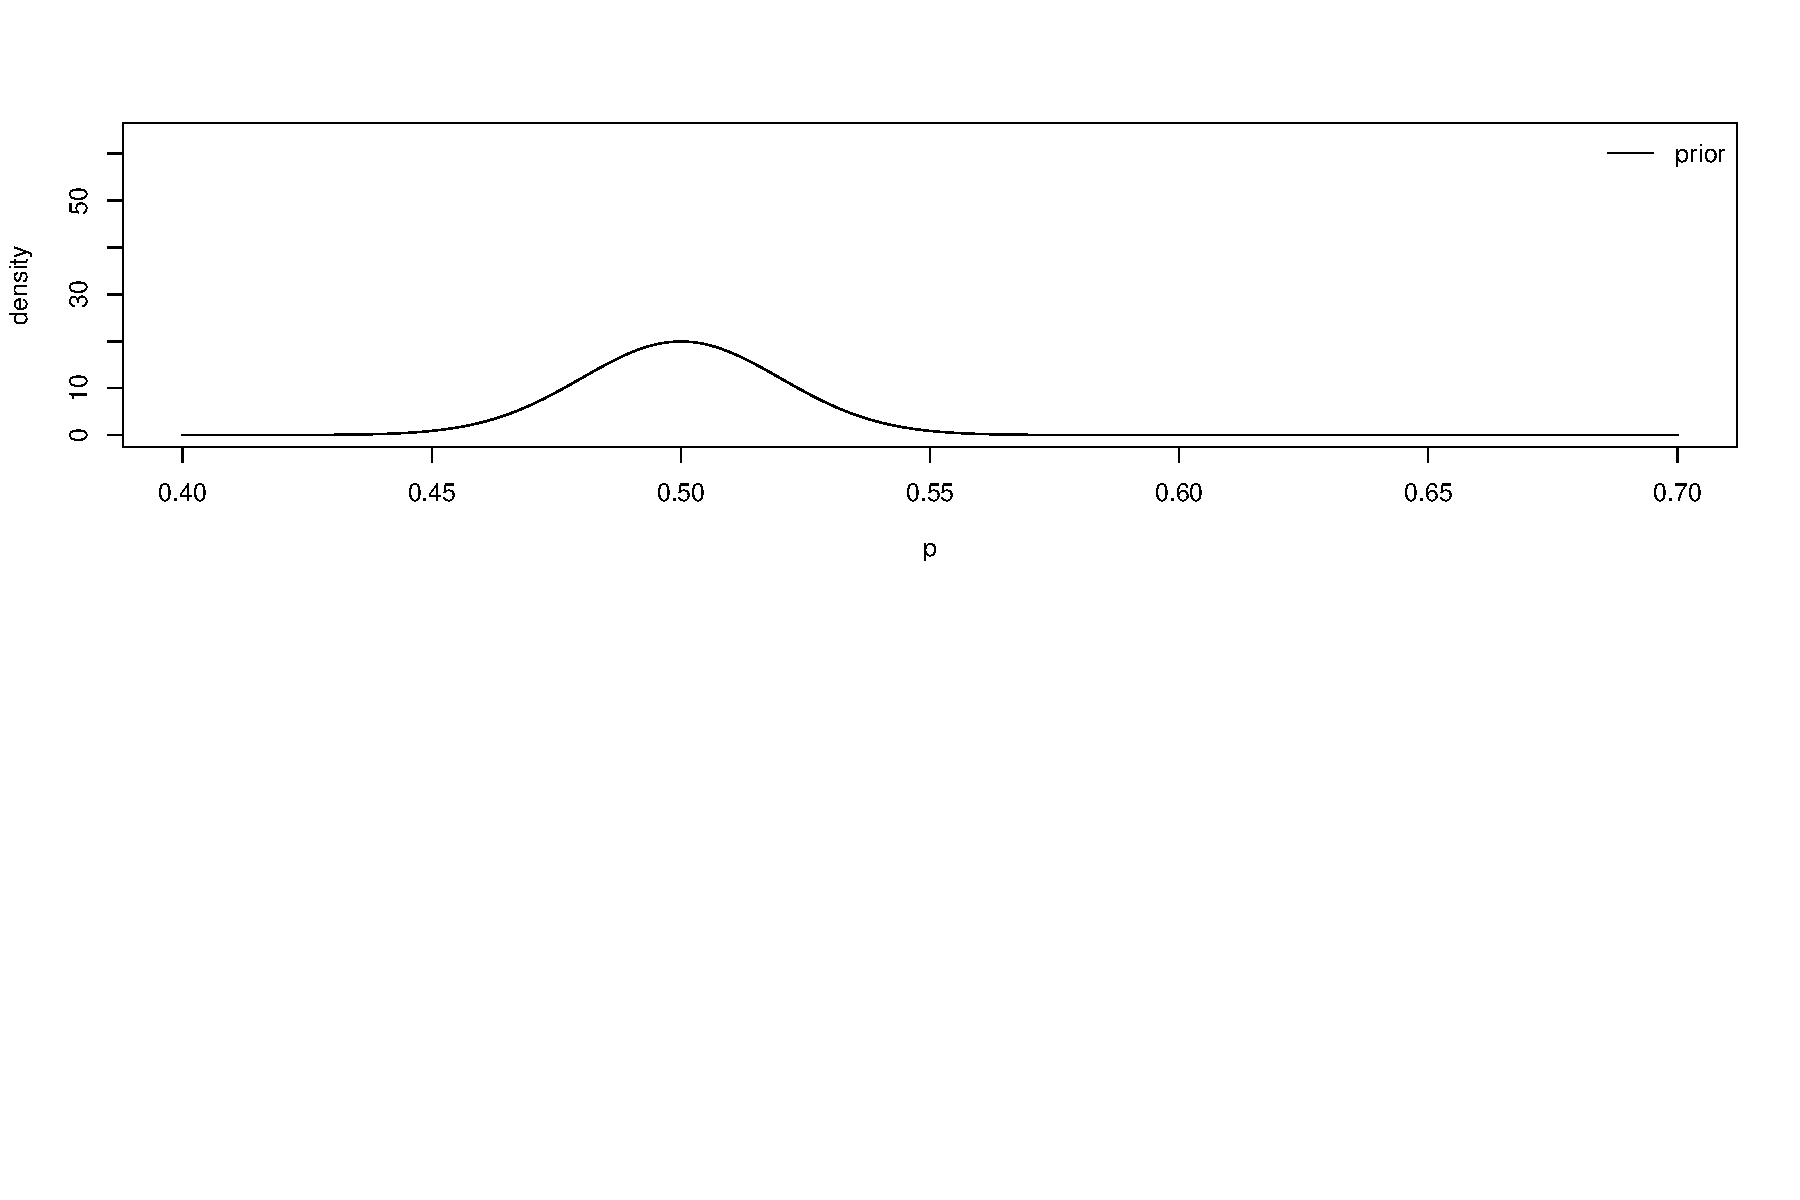
\includegraphics[width=\textwidth]{figure/bayes1.pdf} 
\end{center}

\end{frame}
%------------------------------------------------------------------------------



%------------------------------------------------------------------------------
\begin{frame}
\frametitle{The Bayesian Procedure}
Say we collect data, represented by the red line, suggesting $p=0.6$
\begin{center}
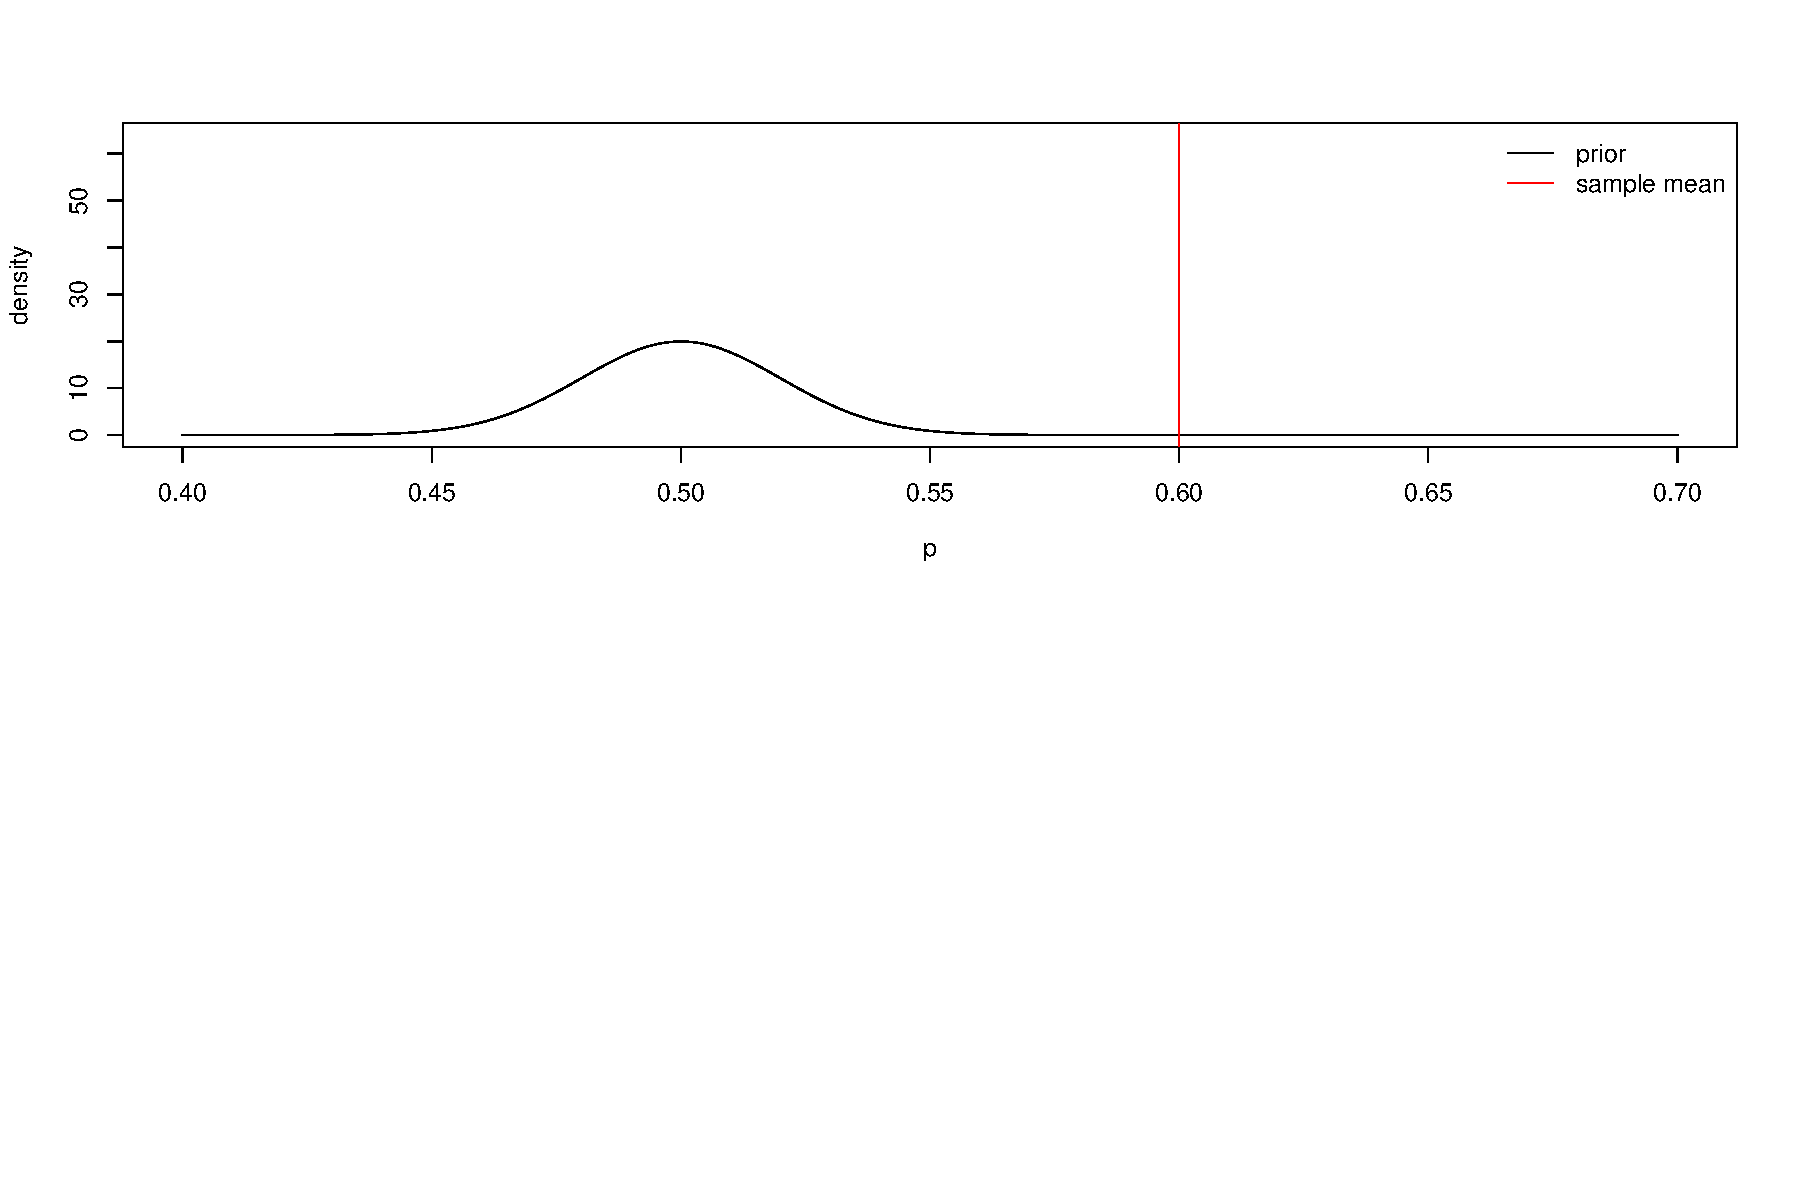
\includegraphics[width=\textwidth]{figure/bayes2.pdf} 
\end{center}

\end{frame}
%------------------------------------------------------------------------------



%------------------------------------------------------------------------------
\begin{frame}
\frametitle{The Bayesian Procedure}
We then \blue{update} our belief, as reflected in the posterior distribution!
\begin{center}
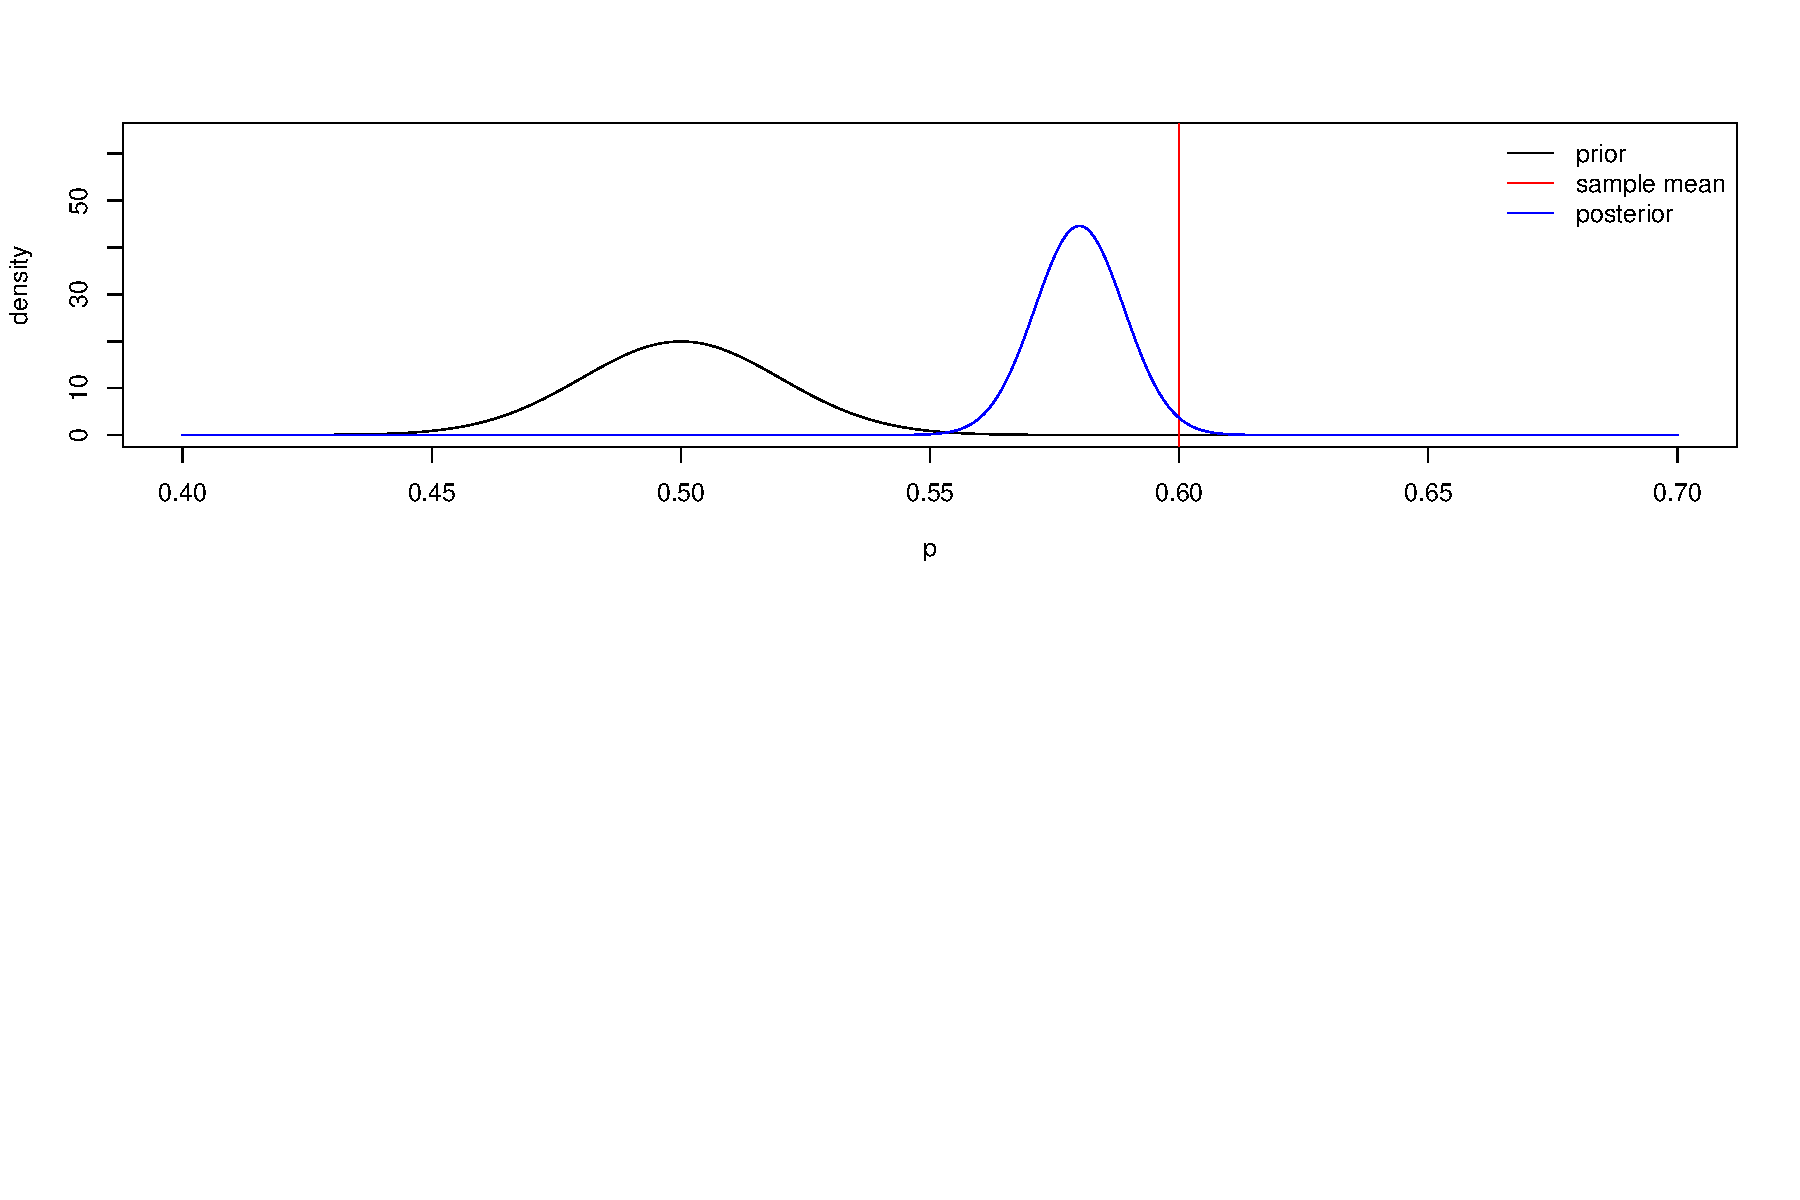
\includegraphics[width=\textwidth]{figure/bayes3.pdf} 
\end{center}

\end{frame}
%------------------------------------------------------------------------------



%------------------------------------------------------------------------------
\begin{frame}
\frametitle{The Bayesian Procedure}
Now say we have a stronger prior belief that $p=0.5$
\begin{center}
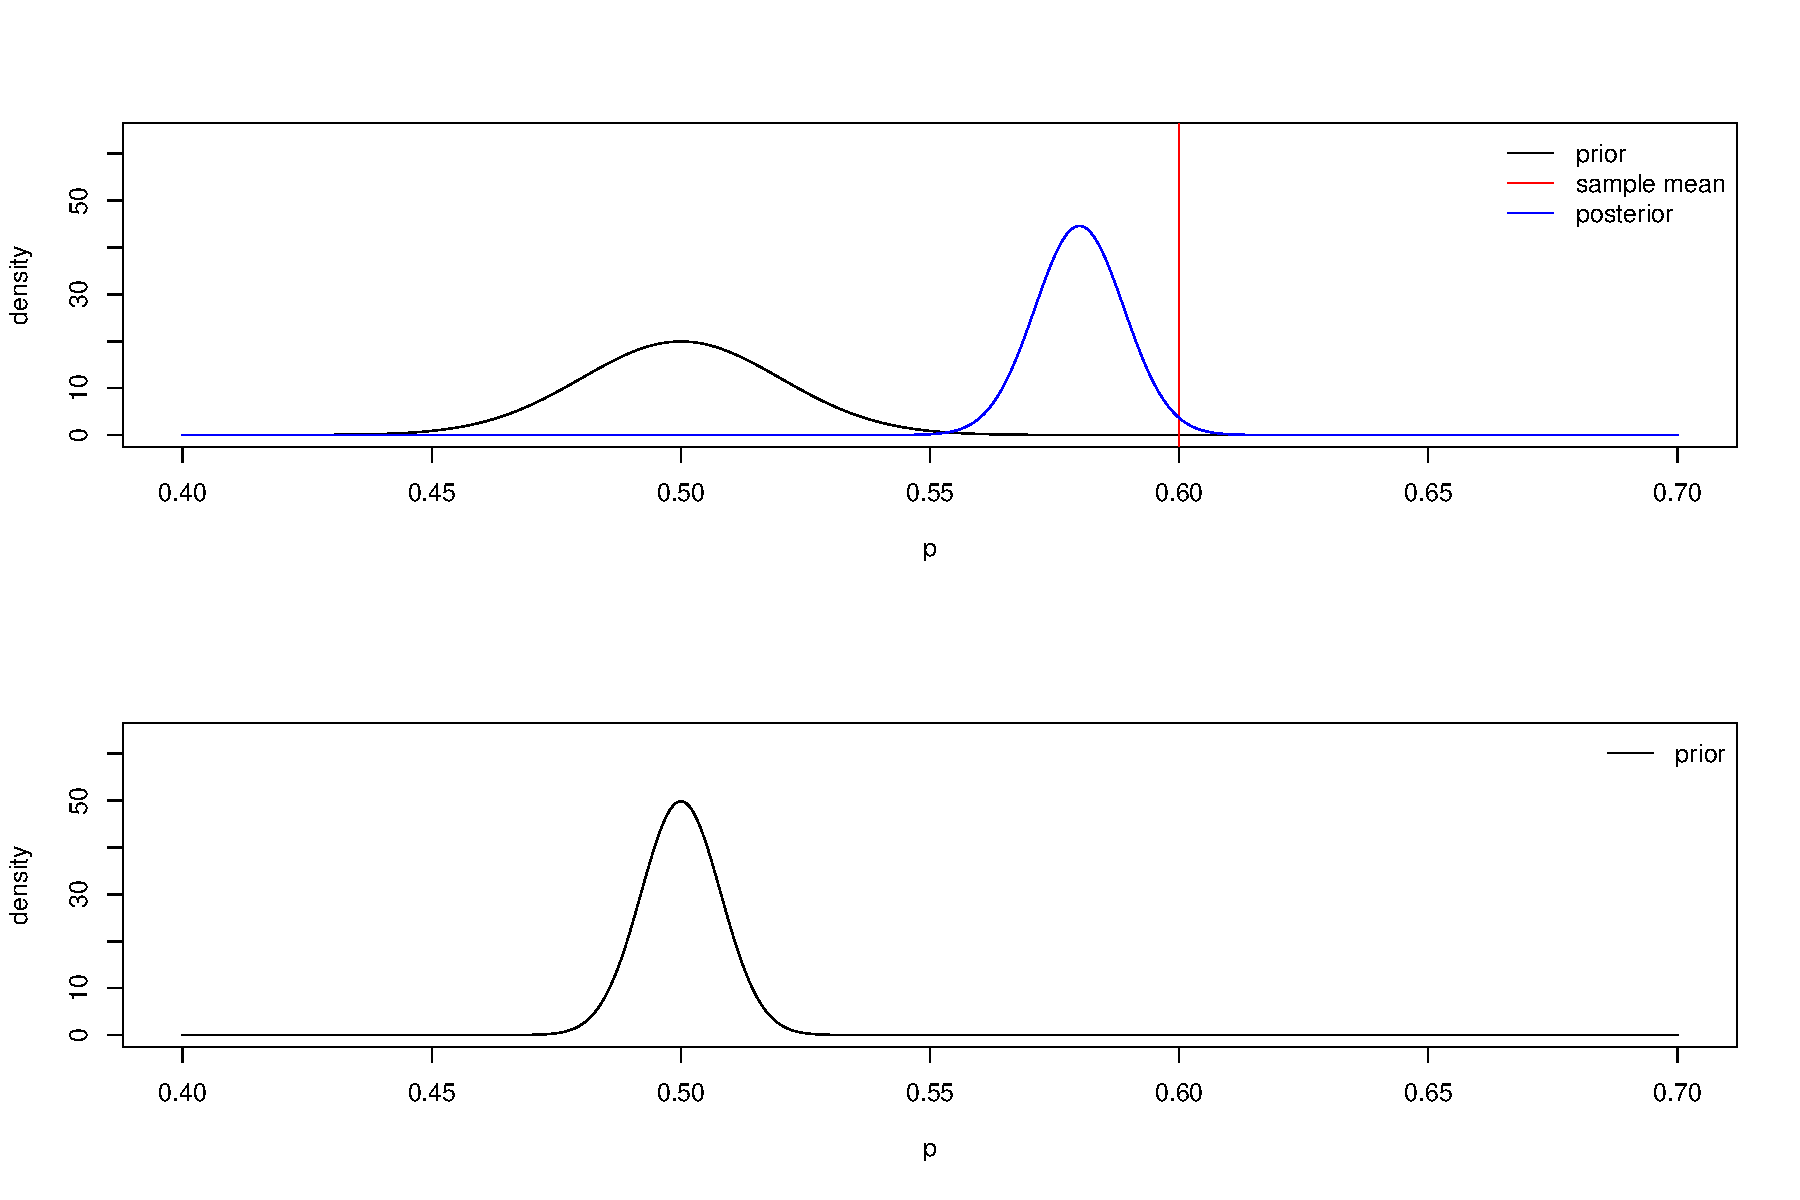
\includegraphics[width=\textwidth]{figure/bayes4.pdf} 
\end{center}

\end{frame}
%------------------------------------------------------------------------------


%------------------------------------------------------------------------------
\begin{frame}
\frametitle{The Bayesian Procedure}
Say we observed the same data (as represented in red).
\begin{center}
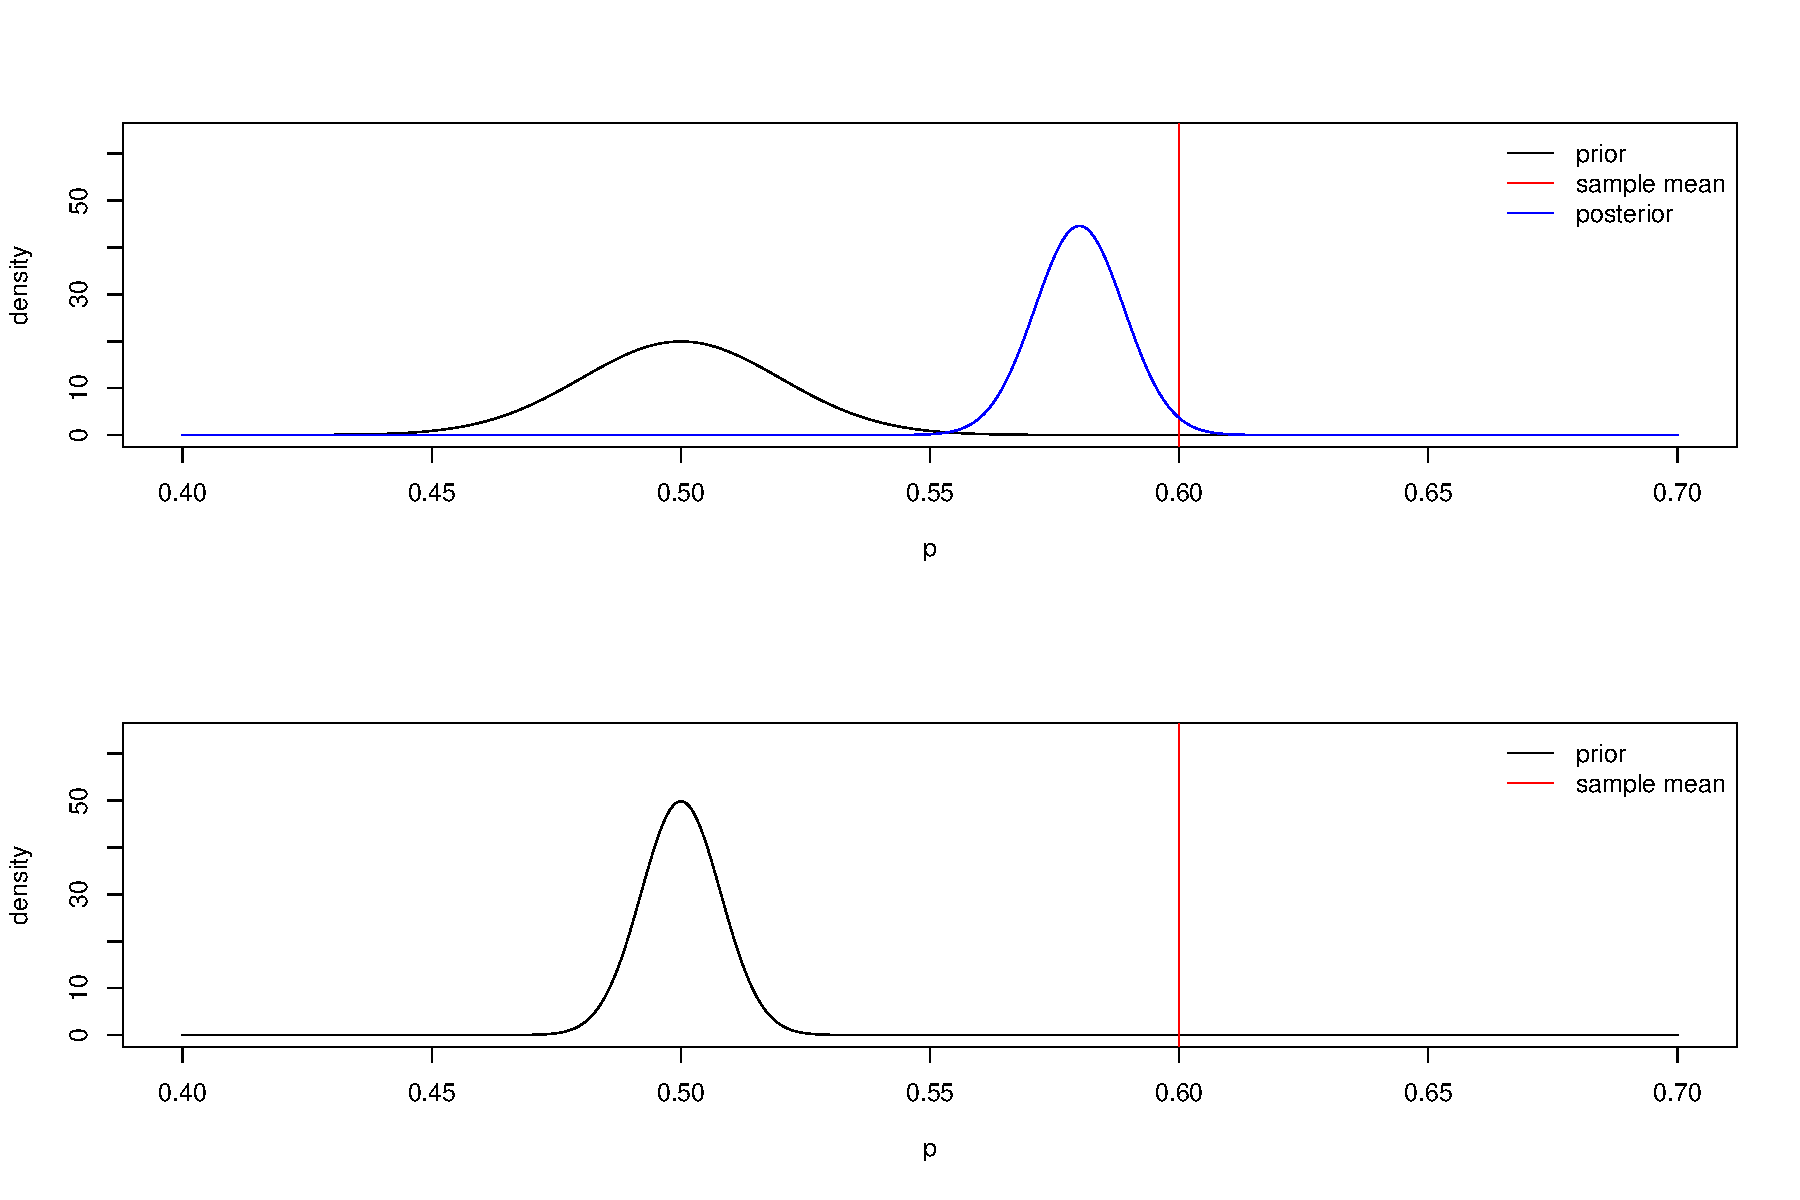
\includegraphics[width=\textwidth]{figure/bayes5.pdf} 
\end{center}

\end{frame}
%------------------------------------------------------------------------------


%------------------------------------------------------------------------------
\begin{frame}
\frametitle{The Bayesian Procedure}
The posterior in this case is pulled left due to the sharper prior.
\begin{center}
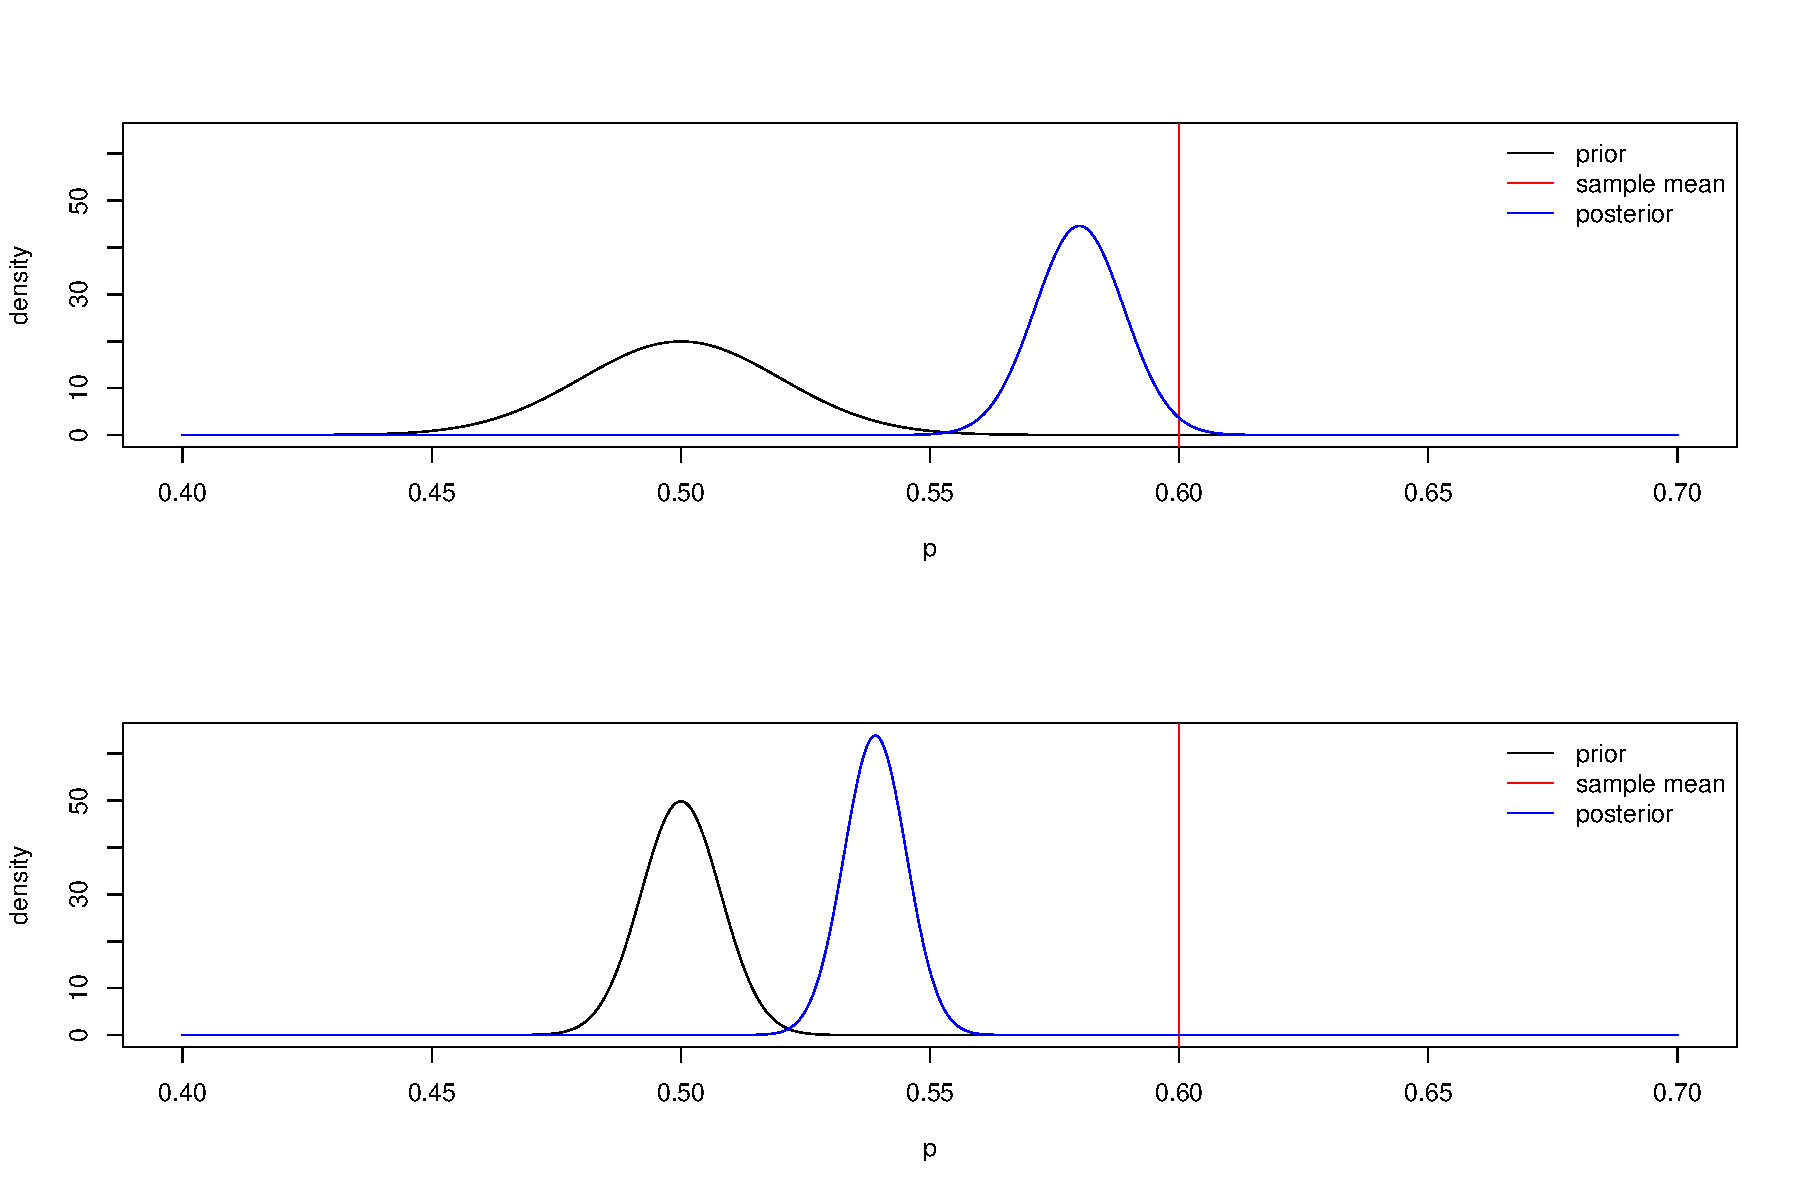
\includegraphics[width=\textwidth]{figure/bayes6.pdf} 
\end{center}

\end{frame}
%------------------------------------------------------------------------------


%------------------------------------------------------------------------------
\begin{frame}
\frametitle{Back to Debate}

Frequentists believe statistics should be completely \blue{objective} and therefore do not accept the premise of a subjective prior.  

\pause\vspace{0.5cm}

Back to Hypothesis Testing Machine example.  In order to use such a procedure in real life, we would need to specify some prior belief $\prob(H_A)$ that $H_A$ is true.  

%\pause\vspace{0.5cm}
%
%The debate rages on...
%\begin{center}
%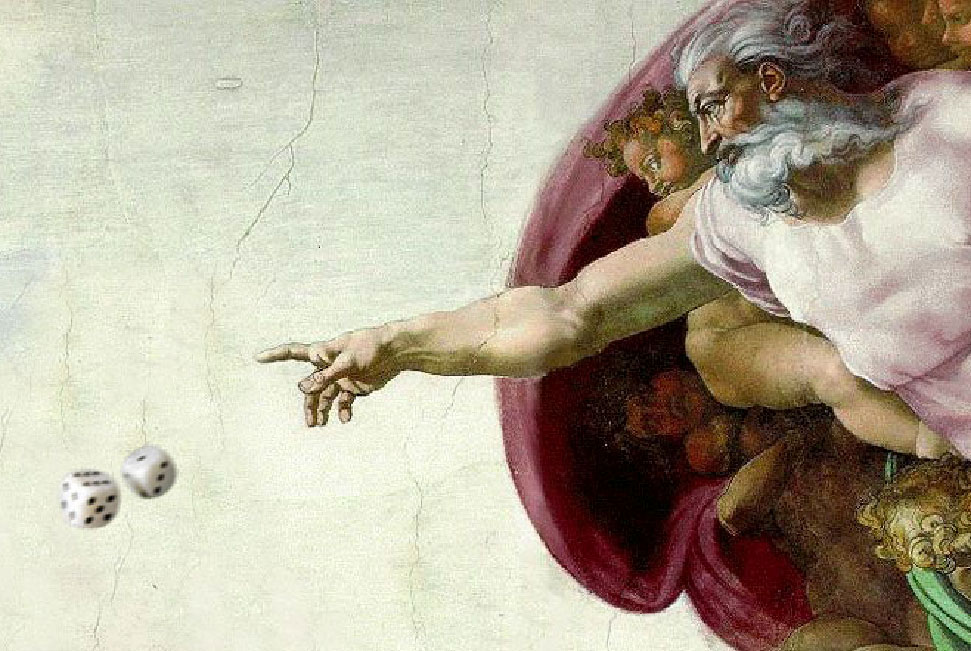
\includegraphics[width=0.6\textwidth]{figure/dice.jpg} 
%\end{center}

\end{frame}
%------------------------------------------------------------------------------



\end{document}










